Este paso del algoritmo consiste en emparejar los objetos de ambas im\'agenes. Esto es muy importante para el seguimiento de objetos que se desplacen en tres dimensiones ya que se necesita la informaci\'on de dos im\'agenes para reconstruir su posici\'on. \\

\begin{figure} [htp]
	\centering
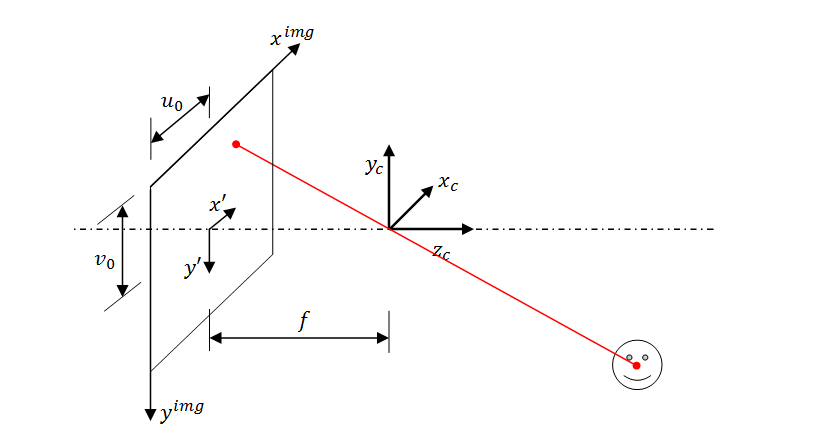
\includegraphics[width=0.75\textwidth,natwidth=544,natheight=388]{../Images/c2/pinhole_model.png} 
	\caption{Modelo Pinhole de C\'amara}
	\label{fig:Pinhole_Model}
\end{figure}

En este art\'iculo se asume que la c\'amara se comporta seg\'un el modelo Pinhole. Adem�s, se asume que el eje de la c\'amara es el eje Z, por lo que cada punto del espacio tiene la siguiente proyecci\'on sobre el plano de la imagen. \\

\begin{equation} \label{eq:pinhole_cam_eq}
\begin{split}
X^{img} = - f*\frac{X}{Z} \\
Y^{img} = f*\frac{Y}{Z}
\end{split}
\end{equation}

Donde $f$ es la distancia focal; Y $X^{img}$ e $Y^{img}$ son las proyecciones del punto dimensional sobre el plano de la imagen. Idealmente, si la segmentaci\'on no tiene errores el par de lineas que forman las proyecciones de los puntos cortan en un solo punto. Sin embargo, al existir errores en la primera etapa del algoritmo se busca la m\'inima distancia entre estas rectas que corresponder� con el objeto original. \\

\begin{figure}[hp]
\centering
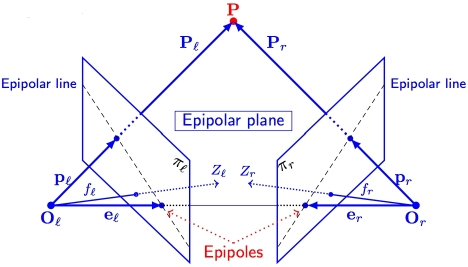
\includegraphics[width=0.75\textwidth,natwidth=468,natheight=267]{../Images/c2/Epipolar_Lines.png}
\caption{Lineas epipolares}
\label{fig:Epipolar_Lines}
\end{figure}

Adem\'as, en las coordenadas de la imagen no existen los valores negativos, por lo que se hace el siguiente cambio de variable (donde $(u_0, v_0)$ es el centroide de la imagen). \\

\begin{align}
X^{img} = u_0 - f*\frac{Y}{X}\\
Y^{img} = v_0 + f*\frac{Z}{X}
\end{align}

Para la minimizaci\'on de la distancia entra las lineas \ref{fig:line-min-dist} usamos las siguiente ecuaciones. \\

\begin{align}
P_1 = P_1^0 + u_1 * s \\
P_2 = P_2^0 + u_2 * t
\end{align}

Siendo  $P_1$ y $P_2$ dos puntos cuales quiera de la l\'inea 1 y 2 respectivamente.

Dados estos dos puntos el segmento que los une $\overline{P_1P_2}$ ser\'a: \\

\begin{equation}
\overline{P_1P_2}=(P_2^0 - P_1^0) + (u_2 * t - u_1 * s)
\end{equation}

Y por \'ultimo, la distancia m\'inima entre ambos (El segmento perpendicular a ambas rectas) es matem\'aticamente: $\overline{P_1P_2} * u1 = 0$ y $\overline{P_1P_2} * u2 = 0$:

\begin{align}
s = \frac{\frac{u_2 * u_2}{u_2 * u_1}*(P_2 - P_1) * u_1 - (P_2 - P_1) * u_2}{\frac{u_2 * u_2}{u_2 * u_1}(u_1 * u_1) - u_1*u_2}	\\
t = \frac{u_1 *_u1 * s - [P_2 - P_1] * u_1}{u_2 * u_1}
\end{align}

Finalmente, $dist(r_1,r_2) = norm(\overline{P_1P_2(s,t)})$.

\begin{figure}[htp]
\centering
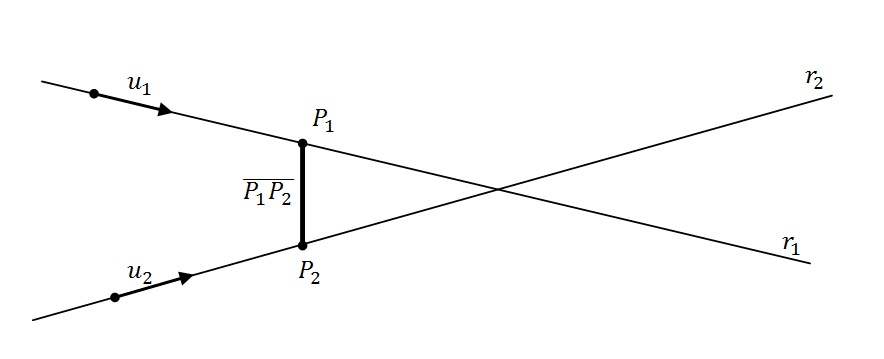
\includegraphics[width=0.7\linewidth]{../Images/c2/line_cut}
\caption{Segmento de m\'inima distancia}
\label{fig:line-min-dist}
\end{figure}


